\begin{figure}[t]
{\small
\begin{verbatim}
   float->float filter MovingAverage(int N) {
     float[N] weights;  // a filter field

     // init function initializes the weights
     init {
       for (int i=0; i<N; i++)
         weights[i] = 1/N;
     }

     // work function declares push, pop, peek rates
     work push 1 pop 1 peek N {
       float result = 0;  // a local variable
       for (int i=0; i<N; i++) {
         result += weights[i] * peek(i);
       }
       push(result);
       pop();
     }
   } 
\end{verbatim}
\vspace{-12pt}
\caption{Example of a StreamIt filter.\protect\label{fig:filter-example}}}
\vspace{-6pt}
\end{figure}

\mysubsection{The StreamIt Language}
\label{sec:background}

StreamIt~\cite{streamitcc} is an architecture-independent language for
signal processing applications.  The model of computation in StreamIt
is Synchronous Dataflow~\cite{lee87static}, in which independent
filters communicate at fixed rates over FIFO channels.  StreamIt aims
to expose the abundant parallelism and regular communication patterns
in stream programs for the benefit of the compiler.  The optimizations
described in this paper would be infeasible in a general-purpose
language such as C.  As detailed elsewhere~\cite{streamitcc}, C
obscures the high-level structure of a streaming application due to
possible aliasing between autonomous filters, complex modulo
expressions on circular buffers, and interleaving of atomic execution
steps with global control flow.
%There is not enough information in C code to automatically perform the
%high-level transformations that experts use to achieve competitive
%performance.  
In addition, StreamIt offers improved programmer productivity over C
due to its parameterizable and composable stream constructs.

The basic programmable unit in StreamIt is a filter, which executes a
user-defined work function as its atomic execution step; for example,
see the {\tt MovingAverage} filter in Figure~\ref{fig:filter-example}.
Filters communicate with each other using FIFO channels.  On each
execution, a filter consumes ({\it pops}) a fixed number of items from
its input channel and produces ({\it pushes}) a fixed number of items
to its output channel.  A filter can also {\it peek} at a given index
on its input channel without consuming the item; this makes it simple
to write sliding-window applications such as the {\tt MovingAverage}.
The push, pop, and peek rates are declared on the same line as the
work function, thereby enabling the compiler to construct a static
schedule of filter firings~\cite{lee87static}.

Each filter has a distinct address space.  A filter can store two
types of variables: a {\it field} and a {\it local}.  Fields are
declared in the scope of the filter and are preserved across
executions, while locals are declared inside the work function and are
only live within a single execution.  There is also an init function,
run once at the beginning of the program, that can be used to
initialize fields.

StreamIt provides three hierarchical structures for composing filters
into larger stream graphs (see Figure~\ref{fig:structures}).  The {\it
pipeline} construct composes streams in sequence, with the output of
one connected to the input of the next.  The {\it splitjoin} construct
distributes data to a set of parallel streams, which are then joined
together in a roundrobin fashion.  The {\it feedback loop} provides a
mechanism for introducing cycles in the graph.  An example of a
pipeline appears in Figure~\ref{fig:iir-pipeline}.  It contains a
single Infinite Impulse Response (IIR) filter, which could be
implemented as shown at the top of Figure~\ref{fig:opt-seq}.

%%         A filter can store two types of variables - \textit{field} and
%% \textit{local}. Field variables are declared outside of the
%% specific functions (work, prework, init), and can be accessed from
%% anywhere within the filter. Local variables are declared within a
%% specific function, and only have scope within that function. For
%% example, a variable declared within the init function is local,
%% and could not be accessed within the work function. Therefore, the
%% init function is used to initialize field variables.

\mysubsection{State Space Example}
\begin{figure}[t]
\vspace{-18pt}
\begin{singlespace}

~~
\begin{minipage}{0.46in}
{\centering
\psfig{figure=pipeline.eps,width=0.46in} \\
}
\end{minipage} 
~
\begin{minipage}{1.3in}
{\centering
\psfig{figure=splitjoin.eps,width=1.3in} \\
}
\end{minipage}
~
\begin{minipage}{1.02in}
{\centering
\psfig{figure=feedback.eps,width=1.02in} \\
}
\end{minipage}
~~~~~~~~~
\begin{minipage}{3in}
\vspace{36pt}
\psfig{figure=iir-pipeline.eps, width=2.33in}
~~~~
\raisebox{12pt}{\psfig{figure=iir-pipeline2.eps, width=0.46in}}
\end{minipage}
\\ ~ \\ {\protect\small (a) A pipeline. ~~(b) A splitjoin. ~~(c) A feedbackloop.}

\begin{minipage}{3.5in}
\caption{Stream structures supported by StreamIt.
\protect\label{fig:structures}}
\end{minipage}
\begin{minipage}{3in}
\caption{Example pipeline with IIR filter.\protect\label{fig:iir-pipeline}}
\end{minipage}
\vspace{3pt}
\hrule
\vspace{3pt}

\hfill
\begin{minipage}{2.2in}
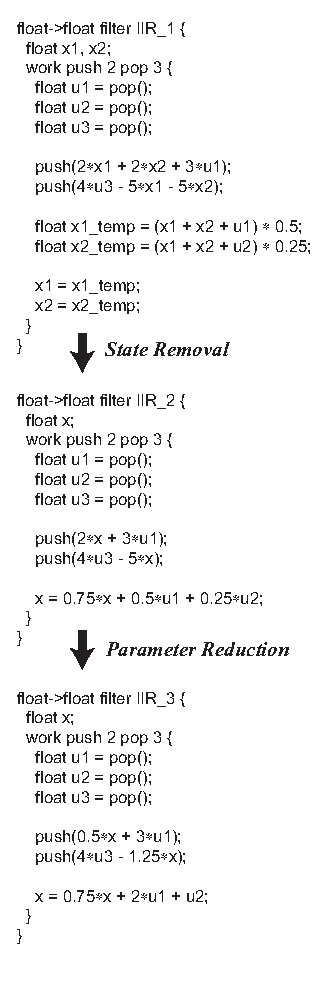
\epsfig{file=statespace-example.eps, width=2.05in}
\end{minipage}
~~~~
\raisebox{10pt}{
\begin{minipage}{3.5in}
Number of multiplications: 8 \\
Number of additions: 8 \\
State space representation:
\begin{eqnarray*}
\small
\vec{\mathbf{y}} & = & \left [ \begin{array} {cc} 2 & 2 \\ -5 & -5
\end{array} \right ] \vec{\mathbf{x}} + \left [ \begin{array} {ccc} 3 & 0 & 0 \\ 0 & 0 & 4 \end{array} \right
 ] \vec{\mathbf{u}} \\
\vec{\dot{\mathbf{x}}} & = & \left [ \begin{array} {cc} 0.5 & 0.5 \\ 0.25
& 0.25 \end{array} \right ] \vec{\mathbf{x}} + \left [ \begin{array} {ccc} 0.5 & 0 & 0 \\
0 & 0.25 & 0 \end{array} \right ] \vec{\mathbf{u}}
\end{eqnarray*}
\vspace{9pt} ~ \\
\hrule
\vspace{12pt} ~ \\
Number of multiplications: 7 \\
Number of additions: 4 \\
State space representation:
\begin{eqnarray*}
\small
\vec{\mathbf{y}} & = & \left [ \begin{array} {cc} 2 \\ -5
\end{array} \right ] \vec{\mathbf{x}} + \left [ \begin{array} {ccc} 3 & 0 & 0 \\ 0 & 0 & 4 \end{array} \right
 ] \vec{\mathbf{u}} \\
\vec{\dot{\mathbf{x}}} & = & \left [ \begin{array} {cc} 0.75
\end{array} \right ] \vec{\mathbf{x}} + \left [ \begin{array} {ccc} 0.5 & 0.25 & 0 \end{array} \right ] \vec{\mathbf{u}}
\end{eqnarray*}
\vspace{-3pt} ~ \\
\hrule
\vspace{12pt} ~ \\
Number of multiplications: 6 \\
Number of additions: 4 \\
State space representation:
\begin{eqnarray*}
\small
\vec{\mathbf{y}} & = & \left [ \begin{array} {cc} 0.5 \\ -1.25
\end{array} \right ] \vec{\mathbf{x}} + \left [ \begin{array} {ccc} 3 & 0 & 0 \\ 0 & 0 & 4 \end{array} \right
 ] \vec{\mathbf{u}} \\
\vec{\dot{\mathbf{x}}} & = & \left [ \begin{array} {cc} 0.75
\end{array} \right ] \vec{\mathbf{x}} + \left [ \begin{array} {ccc} 2 & 1 & 0 \end{array} \right ] \vec{\mathbf{u}}
\end{eqnarray*}
\end{minipage}}
\end{singlespace}
\begin{center}
\vspace{-24pt}

\caption{Example optimization of an IIR filter using linear state
space analysis.  The top segment shows the original code.  The middle
segment depicts the action of state removal, in which the quantity
$x_1 + x_2$ is replaced by a single variable $x$.  The bottom segment
illustrates parameter reduction, in which the coefficients are
refactored so as to eliminate a multiplication (the coefficient of
$u_2$ becomes 1.)\protect\label{fig:opt-seq}}
\end{center}
\vspace{-12pt}
\end{figure}


As described previously, a linear state space model describes a stream
in which both the outputs and the state values are updated as a linear
combination of the inputs and the previous states.  We use the
following notation to describe such systems:
\starteqnstar 
\vec{\dot{\mathbf{x}}} & = & \mathbf{A}\vec{\mathbf{x}} +
\mathbf{B}\vec{\mathbf{u}} \\
\vec{\mathbf{y}}
& = & \mathbf{C}\vec{\mathbf{x}} + \mathbf{D}\vec{\mathbf{u}}
\doneeqnstar
\noindent In these equations, the state vector is denoted by
$\vec{\mathbf{x}}$, the inputs by $\vec{\mathbf{u}}$, and the outputs
by $\vec{\mathbf{y}}$. $\vec{\dot{\mathbf{x}}}$ represents the new
state vector, i.e., the state vector after it is updated.  The 
\clearpage \noindent 
first equation is for the state updates, while the second equation is
for the outputs.  $\mathbf{A}$, $\mathbf{B}$, $\mathbf{C}$, and
$\mathbf{D}$ are matrices whose dimensions depend on the number of
states, inputs, and outputs.

Figure~\ref{fig:opt-seq} illustrates an optimization sequence for an
IIR filter.  Three versions of the filter are shown: original,
following state removal, and following parameter reduction.  In each
case, the state space representation for the filter is shown on the
right, along with the number of multiplications and additions needed
per execution of the work function.

The state removal optimization identifies that the states $x_1$ and
$x_2$ are always used as part of the expression $x_1 + x_2$.  Thus,
one of the states can be eliminated in favor of a single variable,
$x$, that tracks the value of the sum.  While relatively simple in
this example, such a transformation can be quite subtle when applied
to a large representation (e.g., the result of combining many filters
together.)  State removal can reduce storage requirements as well as
eliminate arithmetic operations (in this example, 1 multiplication and
4 additions).  As described in Section~\ref{sec:state-removal}, state
removal is formulated as a general sequence of matrix operations.

The parameter reduction optimization refactors the coefficients that
operate on the state variables in order to reduce the number of
operations needed.  Following the transformation, $x$ assumes a value
that is twice as large as the original (at any given point of
execution).  However, this change does not affect the output of the
filter, as the coefficients in $\mathbf{A}$ are compensated
accordingly.  The transformation enables two coefficients in
$\mathbf{B}$ and $\mathbf{C}$ to change to a value of 1, thereby
eliminating two multiplication operations.  As described in
Section~\ref{sec:parameter-reduction}, this transformation is also
formulated as a general series of matrix operations.
